%%%%%%%% BEGIN PREAMBLE %%%%%%%%

\documentclass[11pt]{article}
\usepackage{acl2015, latexsym, url, times, amssymb, amsmath, amsfonts, mathtools, pdfpages}

\DeclareMathOperator*{\argmax}{argmax}

%%%%%%%% END PREAMBLE %%%%%%%%
\title{Natural Language Processing\\
Fall 2015 Final Project:\\
Sense Disambiguation with the\\
Na\"ive Bayes Classifier}
\author{Maximillian Dumas}


\begin{document}
\maketitle

\begin{abstract}
This paper examines an attempt to implement the Na\"ive Bayes Classifier algorithm for the purpose of performing the task of Word Sense Disambiguation. In it we will discuss the problem of Word Sense Disambiguation broadly, along with a thorough explanation of the Na\"ive Bayes algorithm. Finally, we will present an implementation of the algorithm in Python and analyze the results of the application of the algorithm and difficulties that arose in its application.
\end{abstract}

\section{Introduction}
An incredibly important aspect of computational understanding of human language is word meaning. Without word meaning, effective interpretation of sentences and texts at large is impossible. The meaning of a word occurrence most concisely is the triple of its part-of-speech, lemma form. We call each unique triple that can be assigned to a word form a \emph{sense} of that word. The information provided to us by identifying the sense of a word is critical in any natural language processing task that requires identifying the precise usage of a word. Examples of tasks where this is the case include text classification, question answering, text summarization, and information extraction.

Knowledge of word sense is thus an essential element in natural language processing, but determining word senses by hand is often impractical. Humans are exceptionally good at determining the senses of words in context, and our language is built around that. However, this makes the task of word sense disambiguation difficult for computers, as our language is full of homonyms and homographs, and many words are often used with specific senses in very subtle ways. Yet computers must be able to parse and understand our words if we are to empower them with our language, and we cannot annotate all texts manually. Thus enters the field of word sense disambiguation, which aims to provide computers with the tools to automatically determine the sense of words in a given context. The desired end result of a word sense disambiguation task is that all words in the input have been assigned a single, correct sense that correctly reflects the text's real meaning.

There are many approaches to word sense disambiguation---in particular, machine learning tasks can be broadly adapted to solve the problem. One of the simpler and more efficient of such methods is the Na\"ive Bayes Classifier, which is a probabilistic method that manages to achieve good results while still remaining fairly simple in implementation.

\section{The Na\"ive Bayes Classifier}
As mentioned previously, humans are highly proficient at identifying the sense of a word in use when provided the context of that word. We identify contextual cues that tell us what a specific word's intended meaning must be. We will call these cues \emph{features}, and they may include anything that allows a reader to narrow down the choices for possible meanings. Two of the most important kinds of features are those that provide local context and those that provide global context. Local context refers to looking at how the word sits in the sentence, namely what words it is neighboring, their parts of speech, etc. Global context is the larger semantic space that the word exists in, like the topic of the sentence, paragraph, or text as whole. Every word in a given corpus can be assigned a vector of features providing this context, which we will denote $F$.

Given a feature set observed for a word $w$, $F(w)$, we can then view the problem of disambiguating word sense from a probabilistic perspective. For all $w$, we are then attempting to choose the sense that is maximally probable, $s^*(w)$, given the observed feature set of $w$. That is:

\begin{equation} \label{eq:fundamental}
\begin{split}
s^*(w) &= \argmax_{s \in S(w)} P(s|F(w)) \\
       &= \argmax_{s \in S(w)} \frac{P(F(w)|s)P(s)}{P(F(w))}
\end{split}
\end{equation}

The second form is derived using Bayes' Formula, hence Na\"ive \emph{Bayes} Classifier. This equation is simple and conceptually effective. But in practice, even the second form is difficult to use---meaningfully computing the probability that a given feature vector will occur requires that that entire feature vector have been encountered for that sense before. For large feature vectors the likelihood of this is extremely low, and requires prohibitively large sets of training data. The Na\"ive Bayes Classifier (NBC) is an attempt to minimize the combinations of the features by making the \emph{na\"ive} assumption that the occurrence of each feature is an independent event. With this assumption, we may say that ${P(F(w)|s) = \prod_{f \in F(w)} P(f|s)}$. This assumption is certainly not always true, and is what gives the NBC its na\"ive qualifier. Indeed this equation is often an approximation at best, but usually it is sufficiently accurate to be usable.

Substituting this value in and removing $P(F(w))$, as it is constant for all $s$ and will not affect which sense is chosen for any given word, we arrive at the Na\"ive Bayes Classifier equation:

\begin{equation} \label{eq:nbc}
s^*(w) = \argmax_{s \in S(w)} P(s|w)\!\!\prod_{f \in F(w)}\!\!P(f|s)
\end{equation}

With this formulation, the primary problem in effectively disambiguating word senses is one of training. Identifying the features that accurately determine word sense and finding sense-tagged corpora that exhibit those features are the primary problems in applying the NBC.

\section{Implementation}
The implementation of the NBC included with this paper was developed in Python 3 and consists primarily of the files \emph{nbc.py}, \emph{trainer.py}, \emph{processor.py}, \emph{features.py}, \emph{baseline.py}, and \emph{output/scorer.py}. Included with the project is a script for quickly running the application, \emph{run.sh}.

The general approach for word sense disambiguation using the NBC has 3 overall steps. These steps are Training, Pre-processing, and Disambiguation. Both the training and pre-processing steps involve feature extraction, and as it is identical in both steps, we will discuss that it separately.

\subsection{Baseline}
An important part of establishing the performance of an algorithm is to determine the most basic implementation that the algorithm should improve upon. We call this the baseline. In our case, we chose to implement a most-frequent-sense selector as our baseline upon which to improve. This algorithm simply trains on a set of sense-annotated data and determines which sense is most common for each word. When disambiguating, the algorithm simply chooses that most-frequent sense for each word.

See Analysis for discussion of the performance of this baseline in relation to the NBC.

\subsection{Training}
With the NBC, training is somewhat more complicated than with our baseline. Calculating the values for our equations requires us to evaluate several parameters. This becomes clearer when we expand the meaning of each probability:

$$P(s|w) = \frac{|\{s \text{ and } w\}|}{|\{w\}|}$$

$$P(f|s) = \frac{|\{f \text{ and } s\}|}{|\{s\}|}$$

Thus we must calculate from our training data the number of occurrences of:

\begin{enumerate}
\itemsep 0em
\item each sense with each word
\item each word
\item each feature with each sense
\item each sense
\end{enumerate}

In our implementation these value are stored in two separate maps, denoted $A$ and $B$. $A$ contains all sense total counts and all sense-feature counts. $B$ contains all word total counts and all word-sense counts. It should be noted that each encountered feature is counted on a \emph{per-value} basis. That is, each distinct feature-value pairing is counted separately, so the feature "lemma" with value "apple" will be counted independently from the feature "lemma" with value "orange". As a result, the feature-set observed for each sense is stored as a map of maps, where a feature name yields a map of values encountered for that feature as keys, with its values being the number of times that value occurred for that feature.

\subsection{Pre-processing}
Discuss POS tagging, tokenizing, lemmatization, sentence chunking.

For meaningful feature extraction, it is helpful to attempt to obtain additional metadata about the input that will be sense-disambiguated. This is called the pre-processing stage, the goal of which to attempt to determine as much data that will be useful for identifying sense-context as possible. To this effect, we utilized the Natural Language Toolkit for lemmatization and part-of-speech tagging. These two basic pieces of information can immediately rule out most plainly incorrect senses from being chosen.

\subsection{Feature Extraction}
Feature extraction is the process of identifying desired features in both the training data and the input data and saving their values. We do this in our implementation in \emph{features.py}. The exact same process of feature extraction is performed in both the training data and the input data.

There are 3 primary types of features in our implementation of the NBC. There are qualifying features, collocation features, and bag-of-words features.

Qualifying features represent features that must be present with the considered word in order for it to possibly receive a given sense. Examples of this are lemma and part-of-speech. If we encounter a word that has a part-of-speech that has never been observed with the given sense, then that sense is immediately disqualified from being applicable to that word.

Collocation features represent features that look for characteristics of the neighbors of the considered word \emph{in position}. Collocation features are the primary tool for determining what the local context the sense occurs in. We used a simple POS collocation feature to map out what parts of speech neighboring words had, to attempt to uniquely determine how each sense fits into a sentence.

Bag-of-words features can be used as a useful heuristic for approximating the global context in which a sense occurs. This type of feature simply indicates weather a specific aspect is present in any of the examined neighbors of the considered word. In our case, we detect the presence of neighboring words in an effort to understand the lexical, and hopefully the topical, context in which a sense occurs. For example, if we regularly detect the word "statistical" around one sense of the word "mean" and "person" around another sense of the word "mean", we can much more accurately determine which sense to use where.

\subsection{Application}
The final task of sense disambiguation is thus reduced to evaluating the NBC formula for each word encountered in the input data.

To do so, for each word, first determine if it occurs in $B$, our map of words to word and sense-word counts. This checks if the word was ever encountered in our training data. If it was not encountered, then we have no applicable training data, so that word is not tagged. If it was encountered, then we retrieve from $B$ the total number of occurrences of that word and the set of all senses that occurred with that word and their counts as they occurred with that word.

We then iterate through each of these senses, and from $A$ retrieve the total number of occurrences of that sense as well as the counts of all of the feature-value pairs that were observed with that sense.

We calculate $P(s|w)$ using this information. Then for each observed feature $f)$ we contribute to the total probability that $P(f|s)$. This is calculated as number of times the feature occurred in the training data with the value observed in the input data over the total number of times the sense occurred in the training data.

Qualifying features have this probability calculated directly: If the feature never occurred with the value present in the input data, then the probability will be $0$. Because all of the contributing probabilities are multiplied, this then means that the chance of that sense being applicable is $0$.

Unlike qualifying features, which must all have been observed in training for the sense to apply, we do not want to require a word to have all observed collocation features and bag-of-words features for that sense in order for it to apply. This is because the amount of training data required to ensure that we accurately cover anywhere close to all possible scenarios in which a sense might occur is prohibitively large. Instead, we apply additive smoothing to the $P(f|s)$ calculations for all non-qualifying features. We chose an $\alpha$ value of $10$, which seemed to give the best results from our testing. With this, the presence or absence of feature-values merely contributes to the overall probability of that sense.

With this, we simply choose the sense which yields the highest probability. This represents the calculation of the NBC formula.

\section{Analysis}
Overall, the accuracy of the Na\"ive Bayes Classifier in our implementation was disappointing and our results were somewhat inconsistent with what we expected. We were unable to identify any features that could be calculated within the scope of the project that significantly improved the accuracy of the sense disambiguation.

We applied the NBC to all files in SemCor, a subset of the Brown corpus, which comprises 660,000 words, 230,000 of which are sense-tagged. It was used as the training data for the algorithm, and versions of the files which were stripped of metadata were used as input. The file used as input was always omitted from the training data for that run.

\emph{See attached charts for detailed results.}

These results were calculated with the following features applied:

\begin{enumerate}
\itemsep 0em
\item Part-of-speech was extracted as a qualifying feature
\item Lemma was was extracted as a qualifying feature
\item Part of speech was extracted as a collocation feature from the preceding and following word.
\item "Near sentence start" was extracted as a bag-of-words feature.
\end{enumerate}

Other features, such as collocations of neighboring words or a bag of words for neighboring words, actually significantly decreased accuracy, probably due to insufficient training data. These features were omitted in the final results run.

\section{Conclusion}
The accuracy of the results obtained from the system were significantly less than we hoped. The difficulty in identifying and successfully extracting features that actually provided meaningful data that improved results was unexpected. This difficulty stemmed from the fact that the Na\"ive Bayes Classifier is difficult to reason about, as a probabilistic method. Choices are made as a unit, the product of a large number of factors that are calculated from large amounts of data. This is why other methods, like Decision Trees, are often preferred when developing Word Sense Disambiguation systems; it is generally easier to understand and follow the choices that those systems make, making tuning easier.

There is also a certain degree of unavoidable error that resulted from the fact that we are inferring the metadata that we in turn use to do word disambiguation, namely part-of-speech tagging and lemmatization. Because these systems all feed into one another they have a cascading error effect. For example, switching to a 23\% more accurate lemmatizer reduced the number of incorrectly matched senses by over half. In practice, around 15\% of incorrectly matched senses were a result of and incorrectly chosen lemma or part-of-speech making it impossible for the correct sense to be chosen.

The most obvious avenue for improvement for our implementation is to identify features that provide more advanced contextual information to the classifier to allow it to make better decisions. One incredibly powerful technique that proved outside of the scope of this project is to identify the topics that word senses apply to. From this we could determine other words in that topic that occur with that sense. We could then construct bag-of-words features for each sense from this data, intrinsically allowing us to much more accurately identify the topical context each word is occurring in. This additional information would allow us to, in a great number of cases, particularly with nouns, immediately disambiguate the sense for a given word. We could obtain this topical supplement to WordNet from WordNet Domains, provided by Fondazione Bruno Kessler.

Other features could certainly be identified, possibly involving calculations of path similarity or using hypernyms and hyponyms as bag-of-words features.

Overall, though we implemented the NBC, its performance is generally unacceptable for confident usage. Too many matches are missed or match incorrectly for us to be able to use the system and derive a usable set of senses that cohesively determine the meaning of the text as a whole. The system would undoubtedly do better with more advanced features, but identifying them was difficult and very time-consuming.
\\
\\
\texttt{\textsc{\large Please see the zip file included with this paper for the entire project code.}}

\clearpage
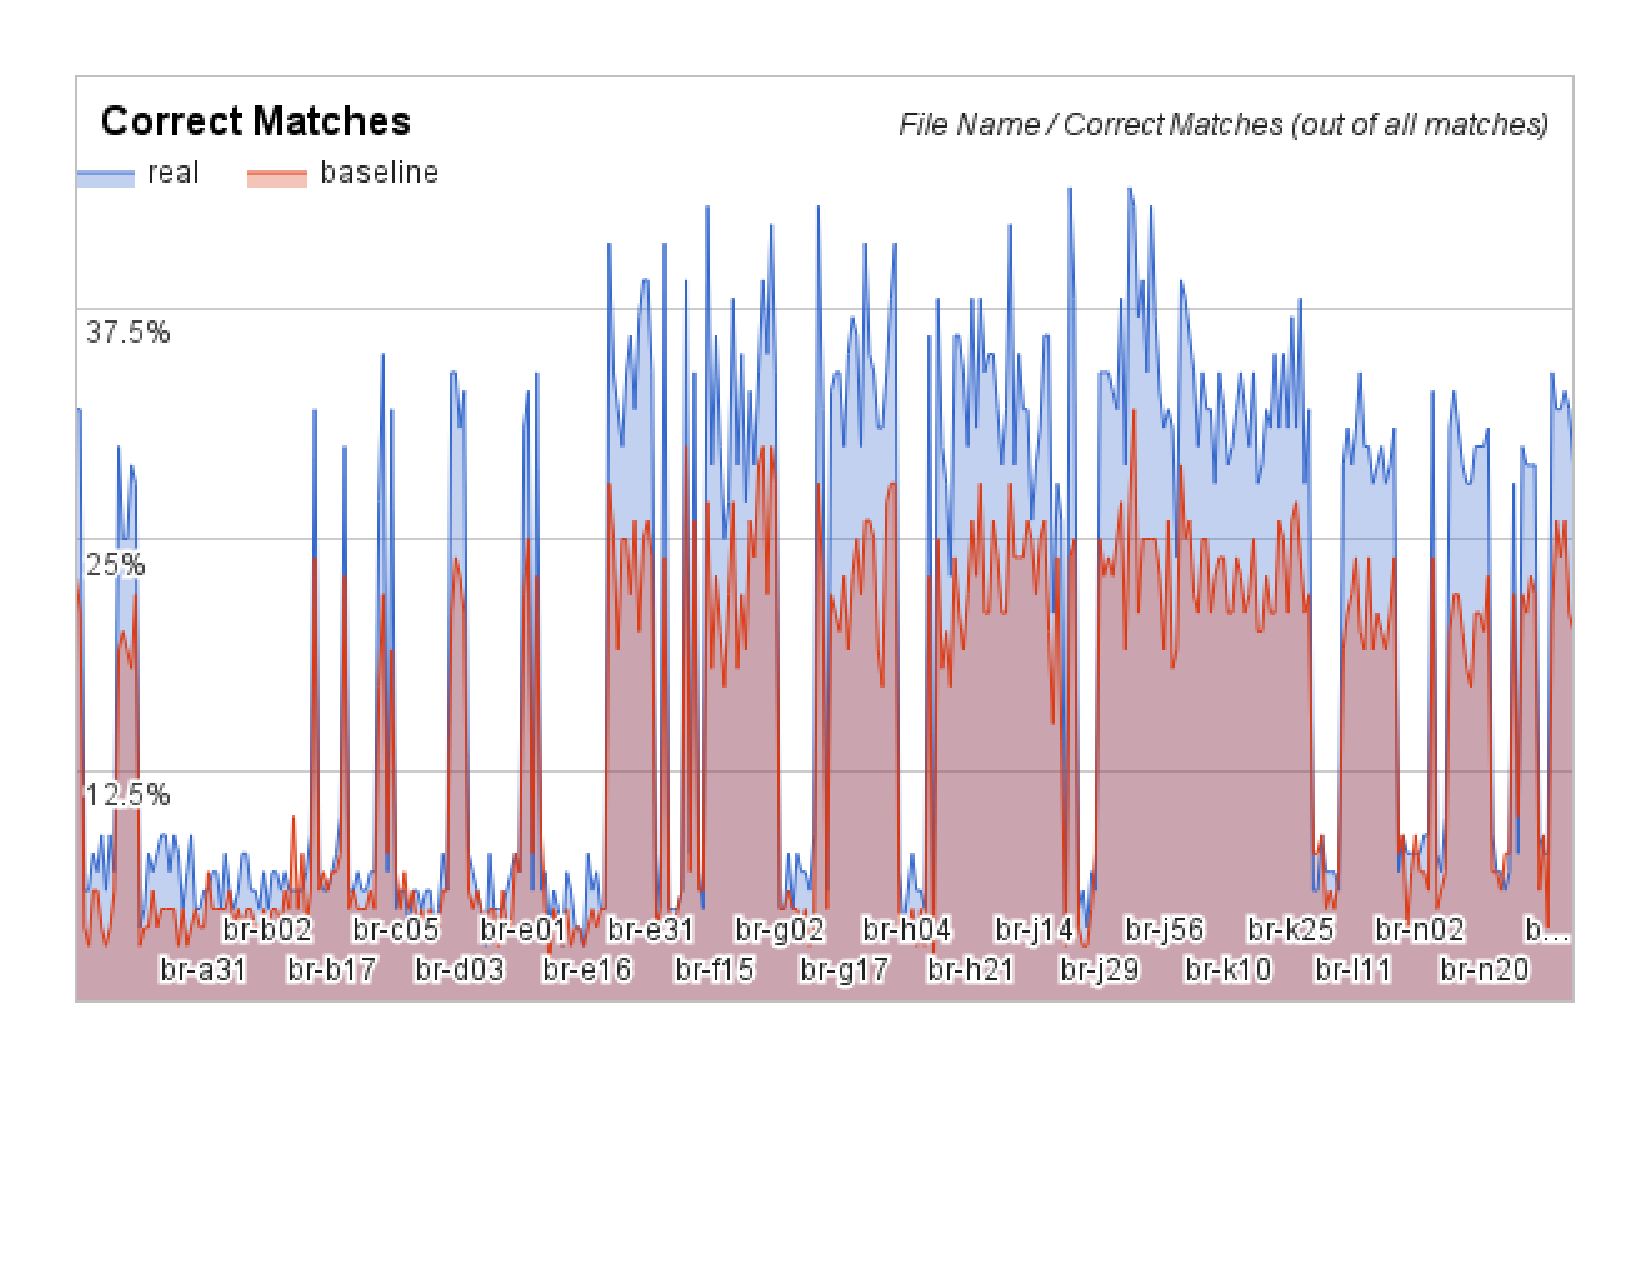
\includepdf[pages=-]{chart_correct.pdf}
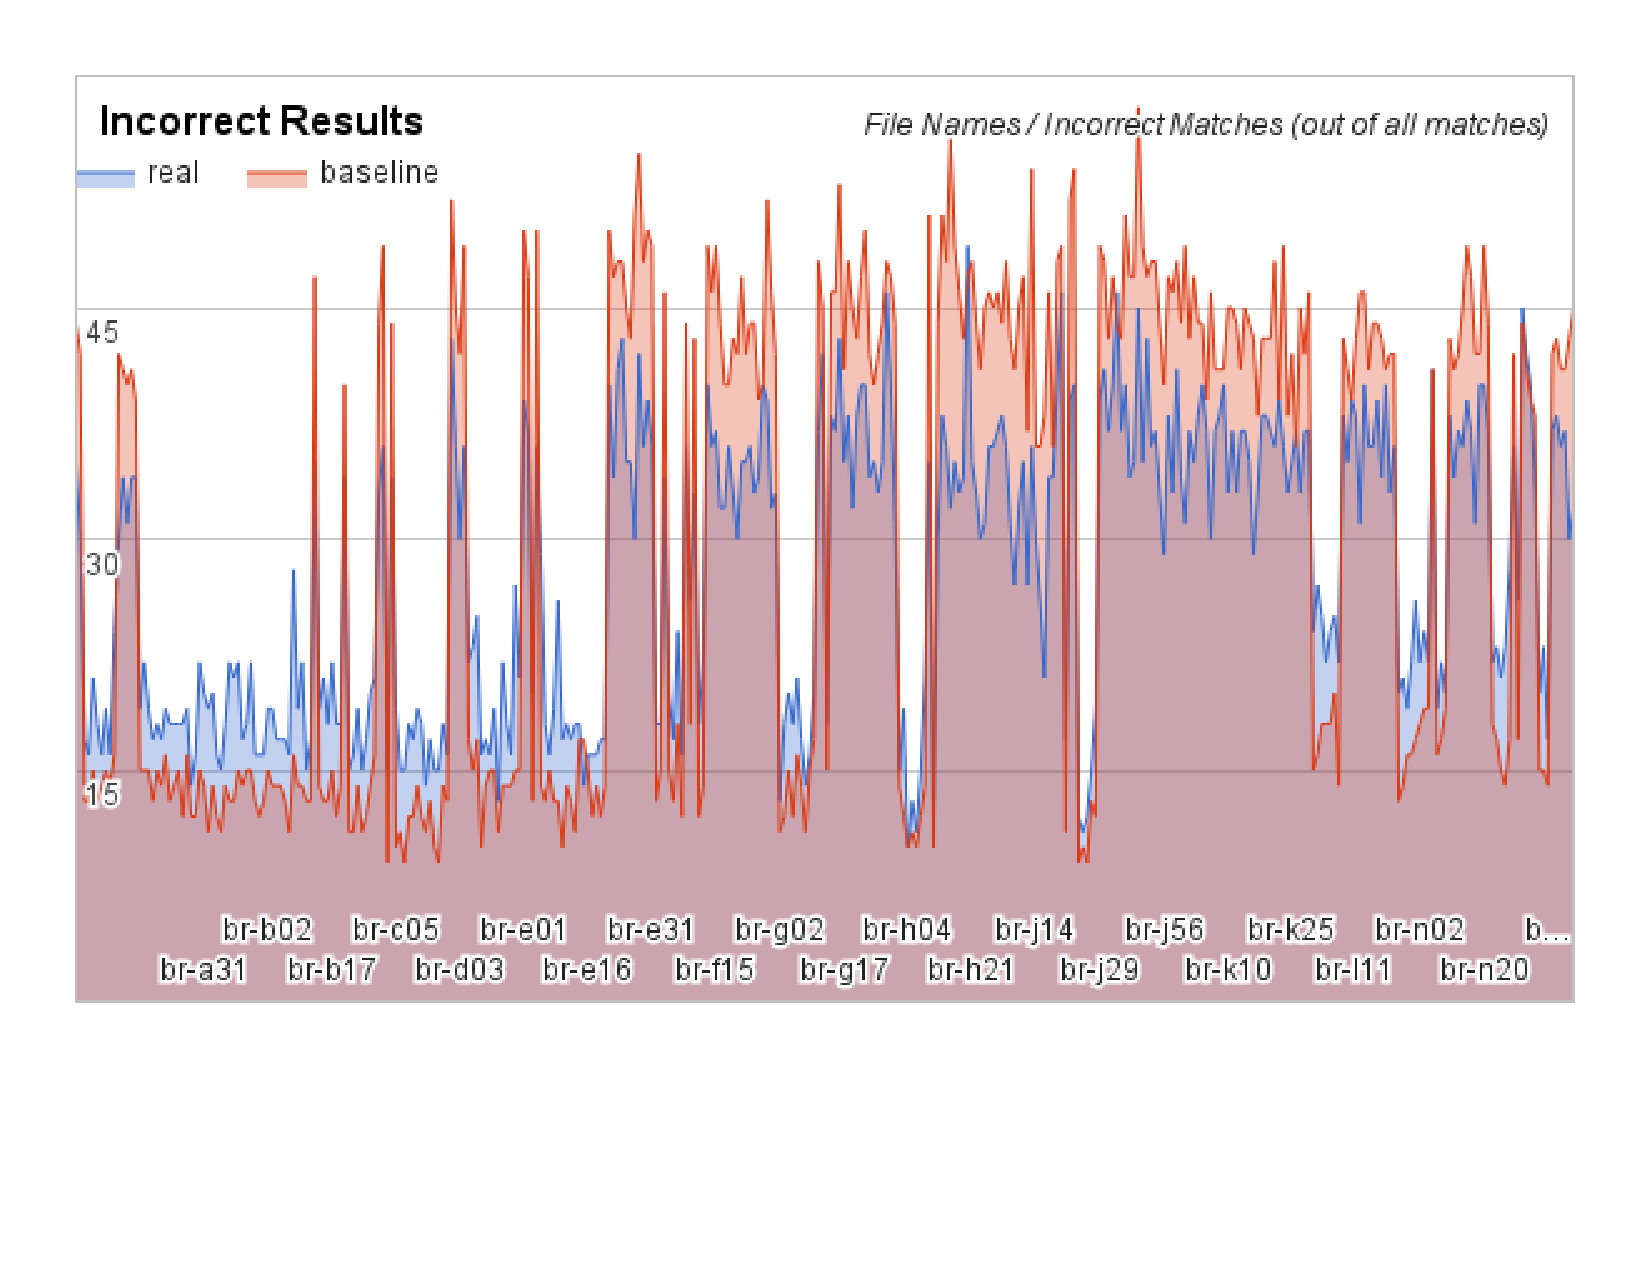
\includepdf[pages=-]{chart_incorrect.pdf}
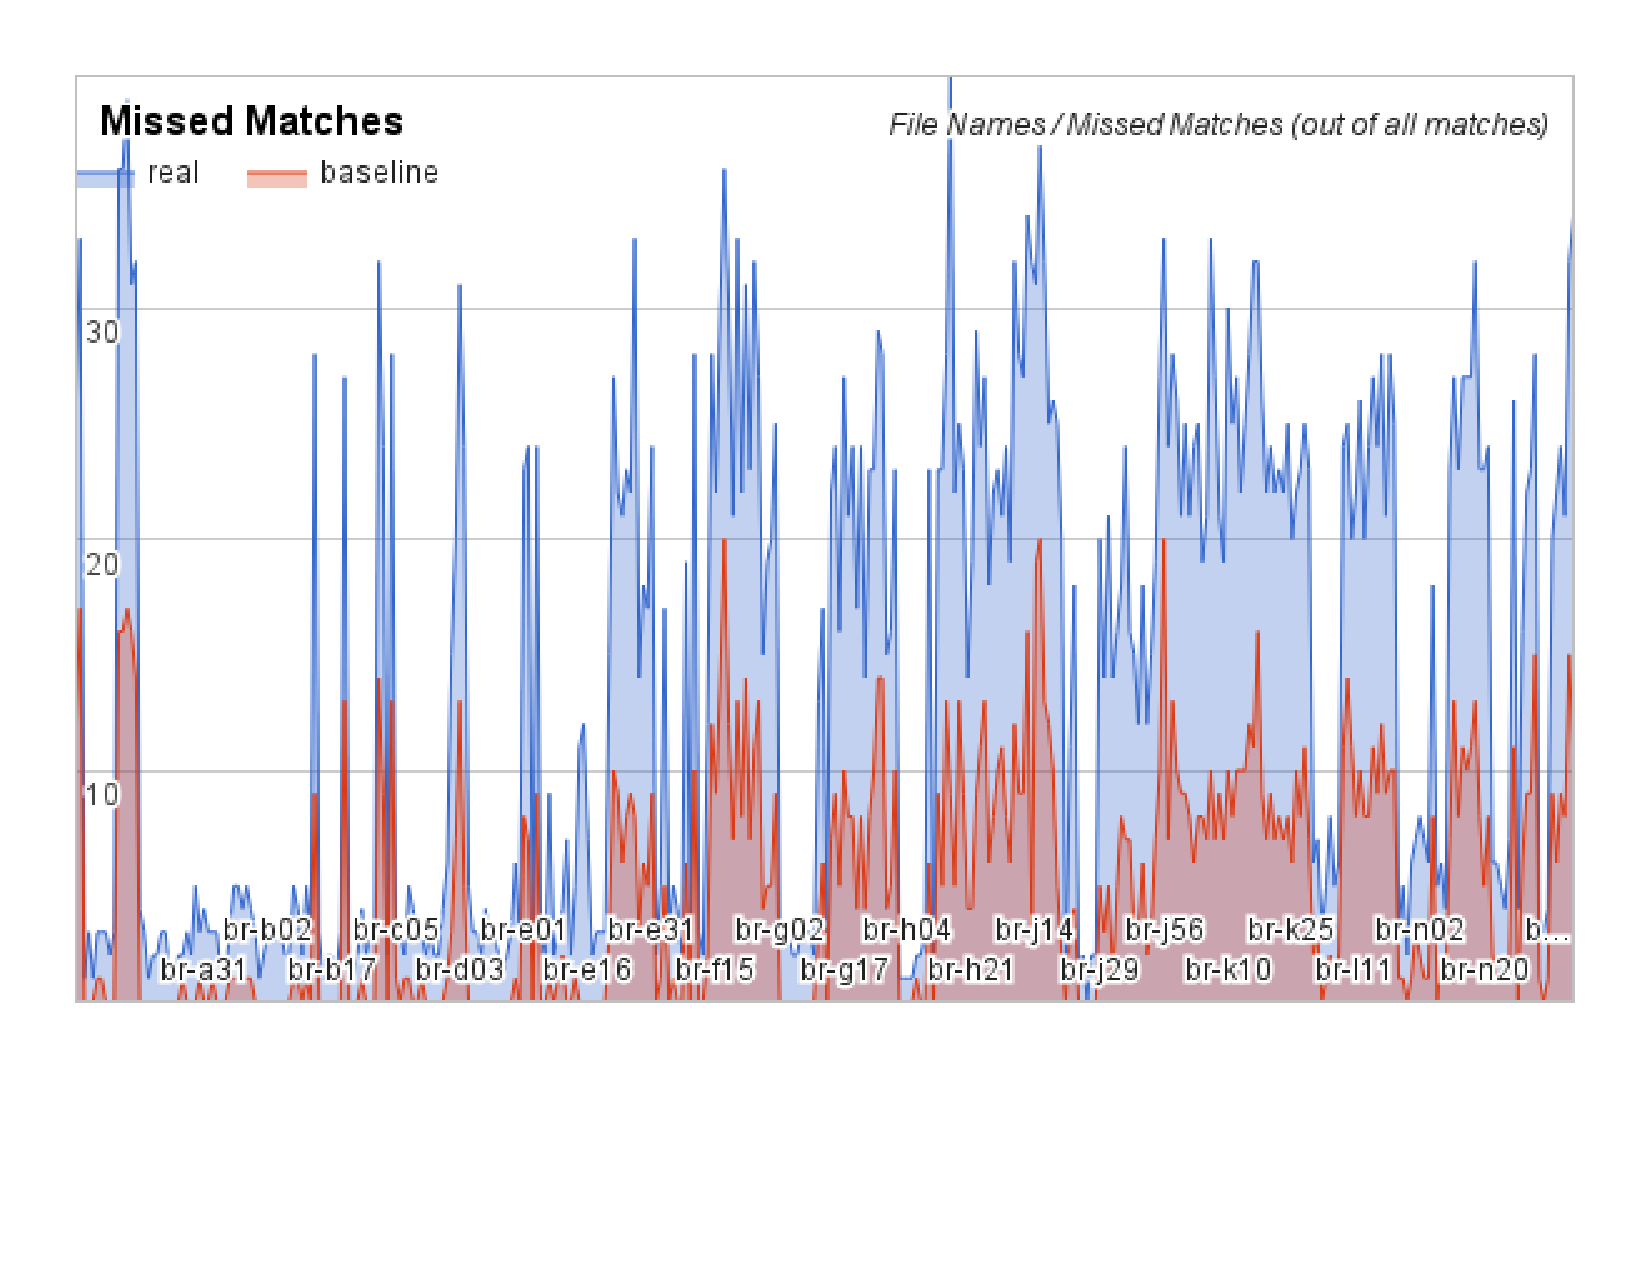
\includepdf[pages=-]{chart_missed.pdf}

\end{document}